% Implicit suffix tree after inserting abbb; bb and b remain implicit.
% Regenerate from this directory:
% latex -interaction=nonstopmode -halt-on-error suffix-tree5.tex
% dvisvgm --no-fonts --exact --bbox=papersize -o suffix-tree5.svg suffix-tree5.dvi
\documentclass[tikz,border=8pt]{standalone}
\usepackage{lmodern}
\usetikzlibrary{arrows.meta}
\definecolor{nodecolor}{HTML}{242A31}
\begin{document}
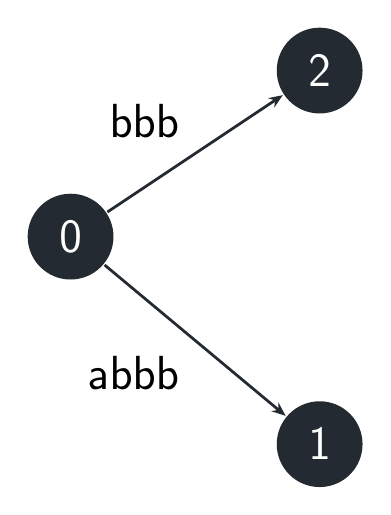
\begin{tikzpicture}[
  x=1pt,y=-1pt,line width=1pt,draw=nodecolor,
  font=\sffamily\fontsize{18}{21}\selectfont,
  vertex/.style={circle,fill=nodecolor,text=white,minimum size=31pt,inner sep=0pt},
  every edge/.style={draw,-{Stealth[length=5pt,width=4pt]}}
]
  \node[vertex] (n0) at (0,0) {0};
  \node[vertex] (n1) at (90,75) {1};
  \node[vertex] (n2) at (90,-60) {2};
  \path
    (n0) edge node[below left=2pt] {abbb} (n1)
    (n0) edge node[above left=2pt] {bbb} (n2);
\end{tikzpicture}
\end{document}
